\documentclass[11pt]{beamer}
\usetheme{Warsaw}
\usepackage[utf8]{inputenc}
\usepackage{amsmath}
\usepackage{amsfonts}
\usepackage{amssymb}
\author{Adam Kaak \\Amira Chehaibi  \\Hechem Ben Farhat \\Mohamed Jaoua \\Mohamed Yahia Bourguiba}
\title{Sujet 7 : Comparaison de deux modèles de mortalité}
\date{Année Universitaire 2020/2021}
\setbeamercovered{transparent} 
%\setbeamertemplate{navigation symbols}{} 
%\logo{} 
%\institute{} 
%\date{} 
%\subject{} 
\begin{document}

\begin{frame}
\titlepage
\end{frame}

%\begin{frame}
%\tableofcontents
%\end{frame}

\begin{frame}{Plan}
\begin{enumerate}
\item Introduction
\item Taux de mortalité 
\item Lecture de données
\item Modèle Lee-Carter
\item Estimation du modèle Lee-Carter
\item Modèle CBD
\item Estimation du modèle CBD
\item Log taux de mortalité de Lee-Carter
\item Procédure par défaut de projection des taux mortalité implémentée dans StMoMo
\item Projection des Taux de mortalité avec forecast
\item Conclusion
\end{enumerate}
\end{frame}

\begin{frame}{Introduction}
L’objectif du projet est d'estimer et de prédire le taux de mortalité des danois agés plus de 50 ans avec 2 modèles différents: 
\begin{itemize}
    \item Le modèle de Lee-Carter.
    \item Le modèle de Cairns Blake Dowd (CBD).
\end{itemize}
\end{frame}

\begin{frame}{Taux de mortalité}
\begin{figure}[!htb]
    \centering
    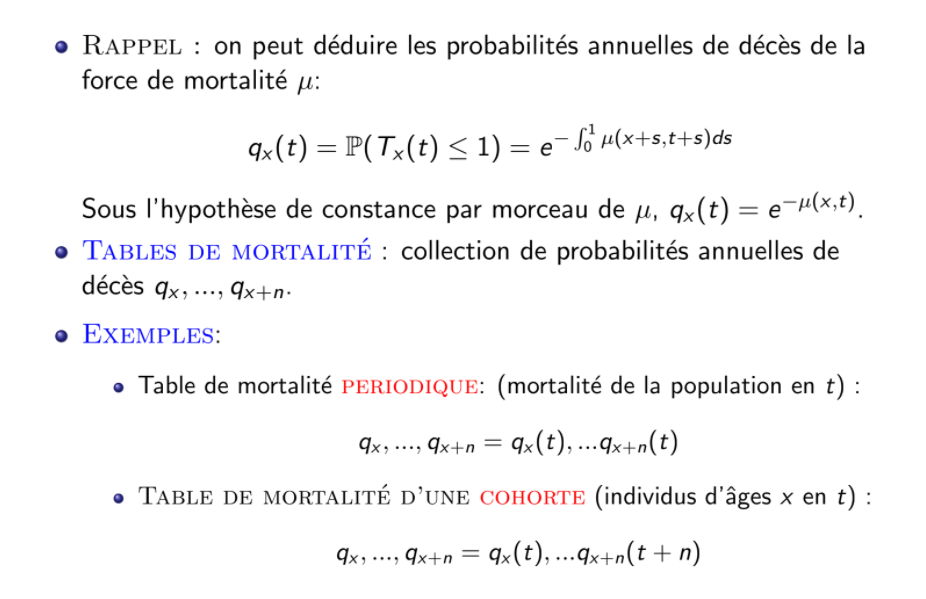
\includegraphics[scale =0.6]{TM.png}
\end{figure}
\end{frame}

\begin{frame}{Lecture de données}
Comme indiqué dans l’énoncé on va travailler sur la population danoise bien évidemment notre pays concerné c’est le Danemark. Pour ce faire nous avons eu recours au site Human Mortality Database (HMD). C’est une base de données qui a été créée pour fournir des données détaillées sur la mortalité et la population aux chercheurs, étudiants, journalistes,
analystes des politiques et autres personnes intéressées par l’histoire de la longévité humaine.
on a utilisé la commande hmd.mx() pour le téléchargement. 
\end{frame}

\begin{frame}{Modèle Lee-Carter}
Modèle:
\begin{figure}[!htb]
    \centering
    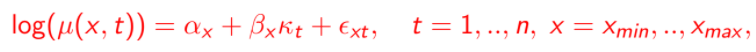
\includegraphics[scale =0.6]{LC1.png}
\end{figure}
avec: 
exp(ax): comportement moyen de la mortalité.
\\kt: Évolution temporelle du taux de mortalité.
\\bx: Vitesse de réduction de la mortalité par age.
\\Les paramètres ne sont pas identifiables:
\begin{figure}[!htb]
    \centering
    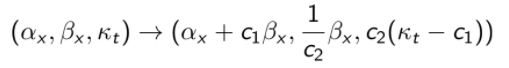
\includegraphics[scale =0.6]{LC2.png}
\end{figure}
Contraintes:
\begin{figure}[!htb]
    \centering
    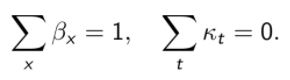
\includegraphics[scale =0.6]{LC3.png}
\end{figure}
\end{frame}

\begin{frame}{Procédure d'estimation Etape 1}
Estimation des paramètres à partir des données historiques.
\begin{figure}[!htb]
    \centering
    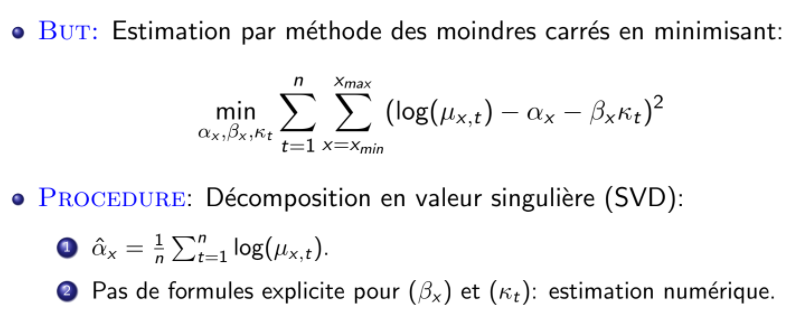
\includegraphics[scale =0.6]{LC5.png}
\end{figure}
\end{frame}

\begin{frame}{Procédure d'estimation Etape 2}
Projection de la force de mortalité future.
\begin{figure}[!htb]
    \centering
    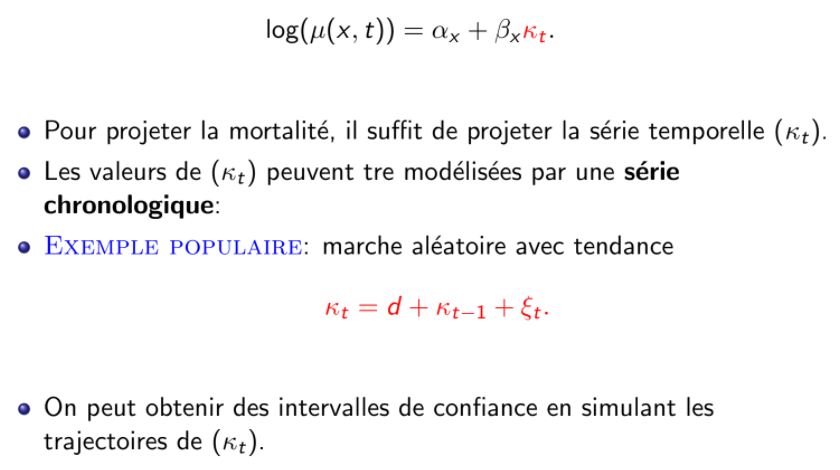
\includegraphics[scale =0.6]{LC6.png}
\end{figure}
\end{frame}


\begin{frame}{Estimation du Modèle Lee-Carter}
\begin{figure}[!htb]
    \centering
    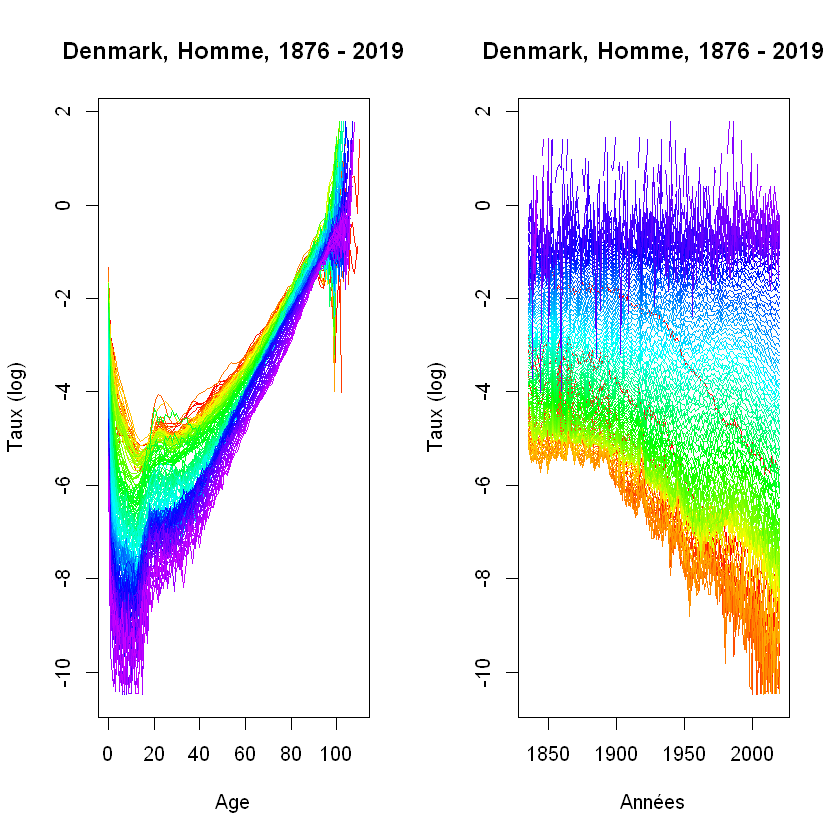
\includegraphics[scale =0.5]{output_7_0.png}
\end{figure}
\end{frame}

\begin{frame}{Estimation du Modèle Lee-Carter}
\begin{figure}[!htb]
    \centering
    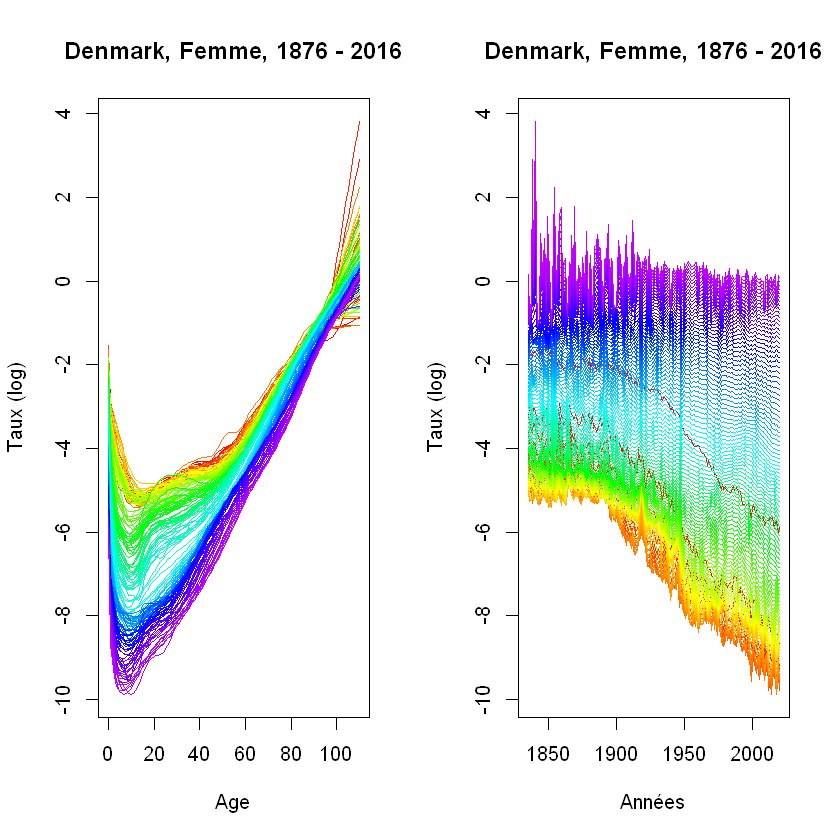
\includegraphics[scale =0.5]{output_7_1.png}
\end{figure}
\end{frame}

\begin{frame}{Estimation du Modèle Lee-Carter}
\begin{figure}[!htb]
    \centering
    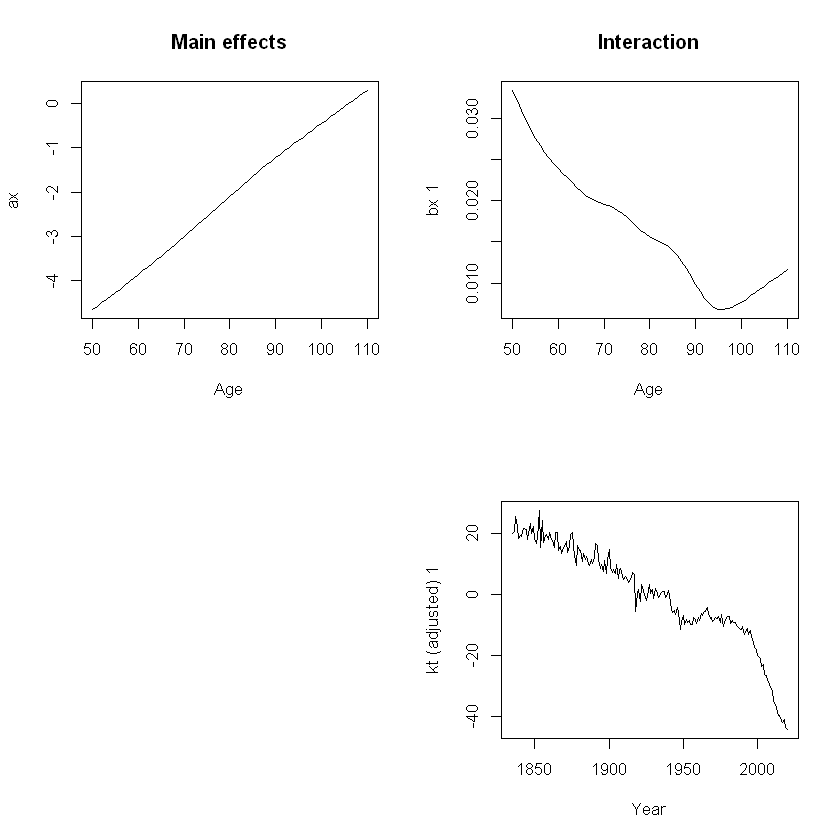
\includegraphics[scale =0.5]{output_7_3.png}
\end{figure}
\end{frame}

\begin{frame}{Estimation du Modèle Lee-Carter}
\begin{figure}[!htb]
    \centering
    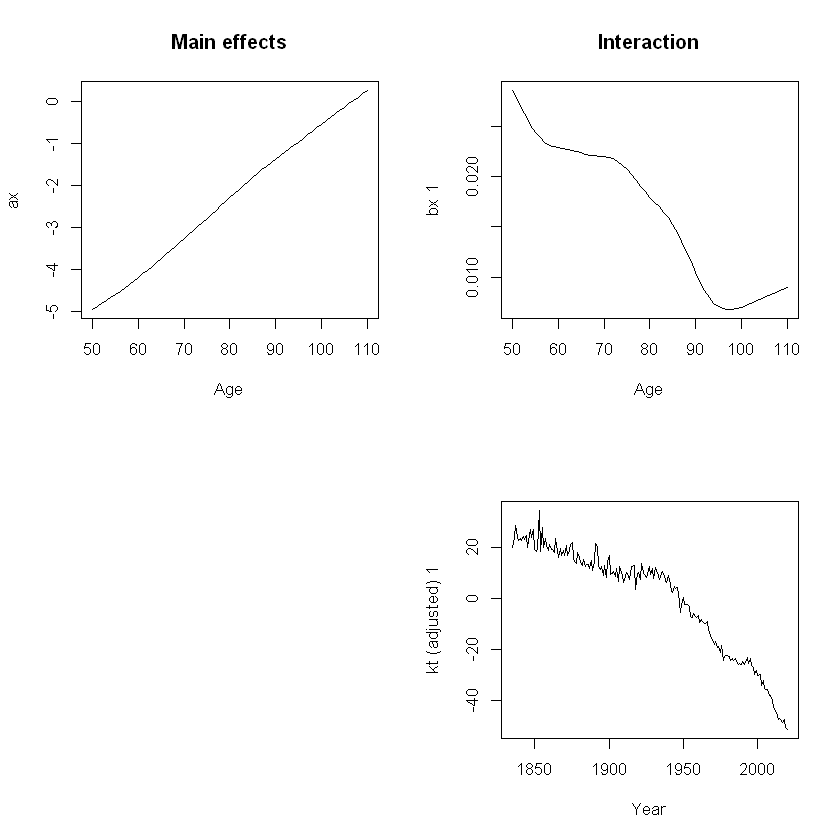
\includegraphics[scale =0.5]{output_7_5.png}
\end{figure}
\end{frame}

\begin{frame}{Estimation du Modèle Lee-Carter}
\begin{figure}[!htb]
    \centering
    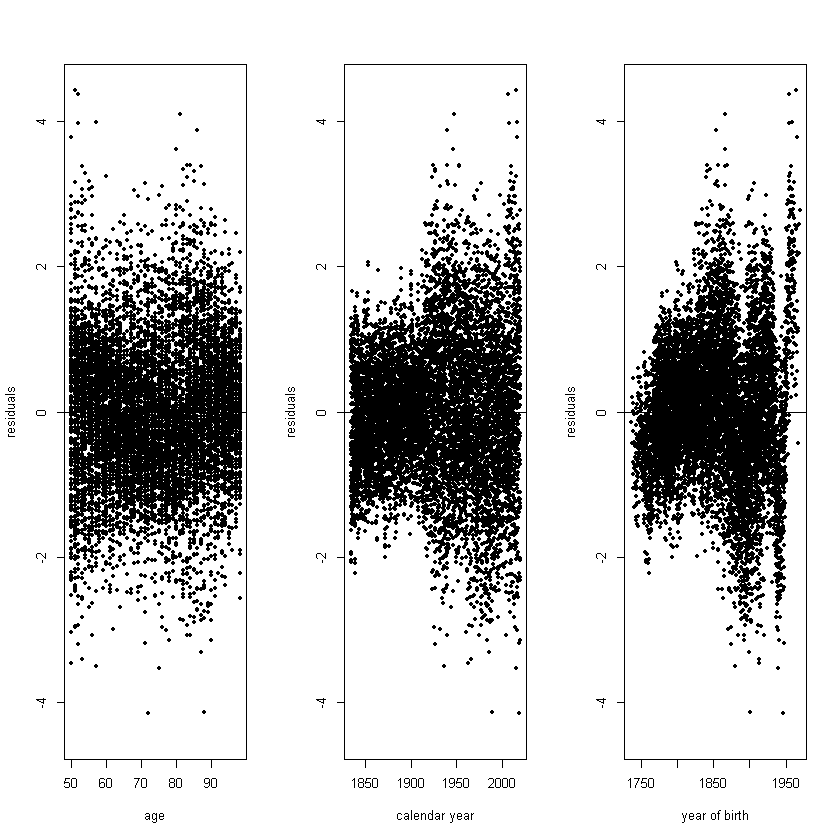
\includegraphics[scale =0.5]{output_9_1.png}
\end{figure}
\end{frame}

\begin{frame}{Estimation du Modèle Lee-Carter}
\begin{figure}[!htb]
    \centering
    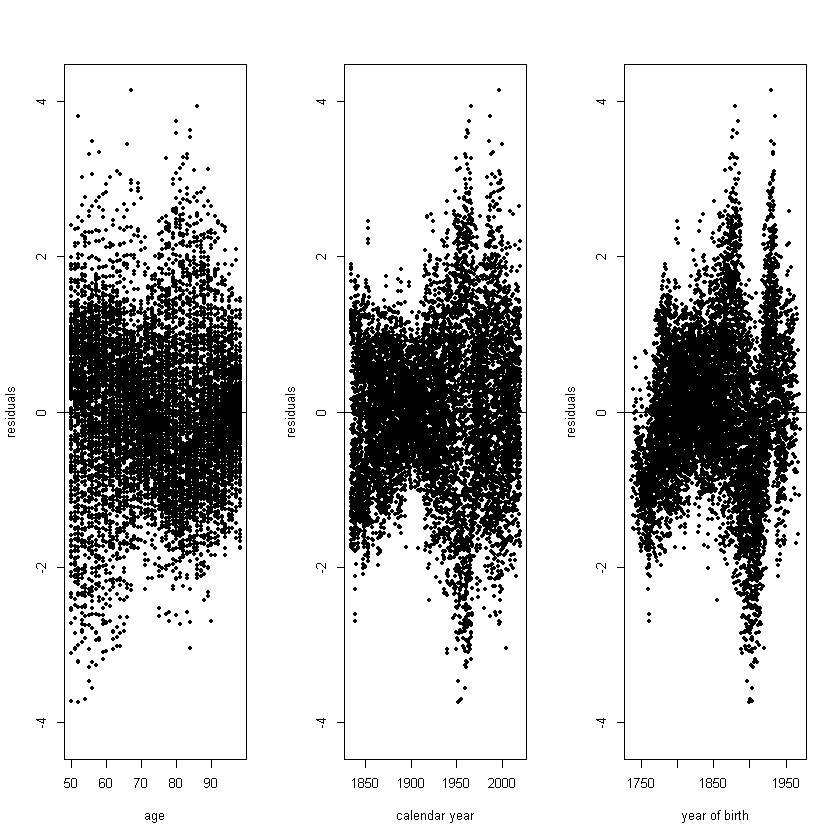
\includegraphics[scale =0.5]{output_11_0.png}
\end{figure}
\end{frame}

\begin{frame}{Modèle Cairns Blake Dowd}
C'est l’une des variantes les plus importantes du modèle Lee-Carter.Il se repose sur la linéarité de la logit des probabilités de décès d’un an à des âges plus avancés.
\begin{figure}[!htb]
    \centering
    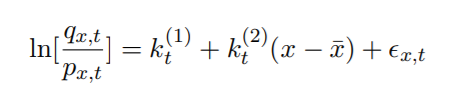
\includegraphics[scale =0.6]{CBD1.png}
\end{figure}
ou Kt(1) et Kt(2) sont deux processus stochastiques et représentent les deux indices temporels du modèle;
\\qx,t et px,t représentent respectivement le décès et la probabilité de survie au temps t pour un individu agé de x;
\end{frame}

\begin{frame}{Estimation du Modèle CBD}
\begin{figure}[!htb]
    \centering
    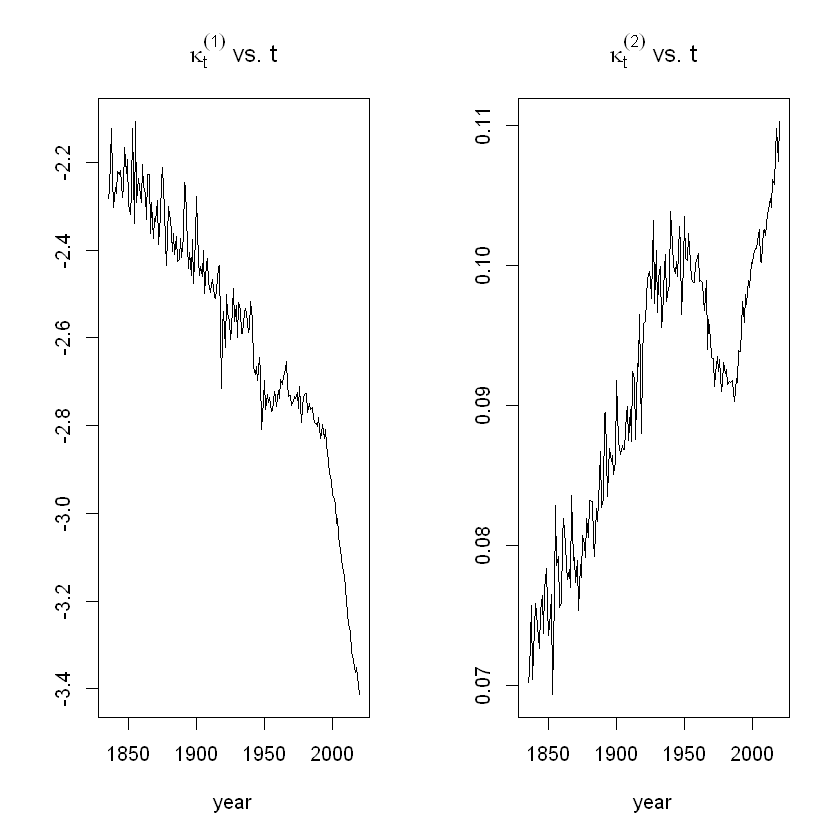
\includegraphics[scale =0.5]{output_18_7.png}
\end{figure}
\end{frame}

\begin{frame}{Estimation du Modèle CBD}
\begin{figure}[!htb]
    \centering
    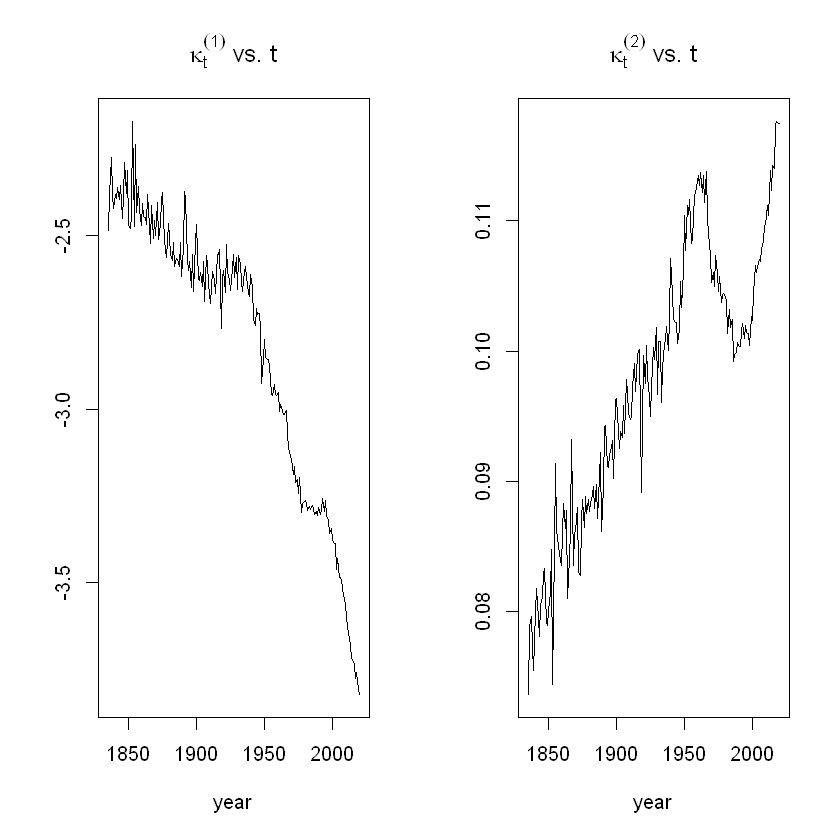
\includegraphics[scale =0.5]{output_18_9.png}
\end{figure}
\end{frame}

\begin{frame}{Log taux de mortalité de Lee-Carter }
\begin{figure}[!htb]
    \centering
    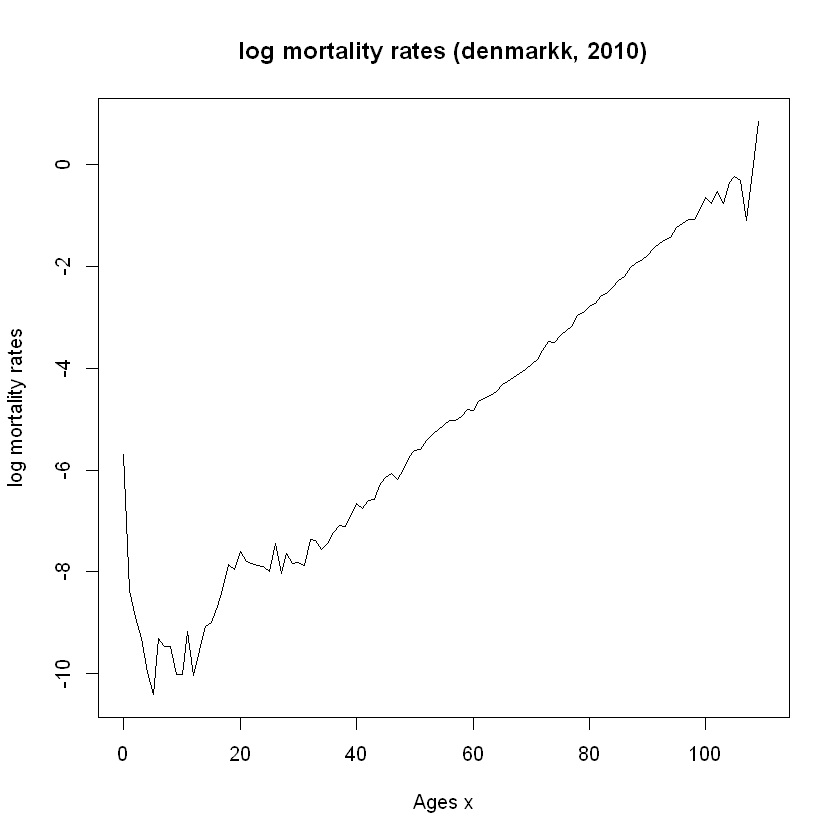
\includegraphics[scale =0.5]{output_20_0.png}
\end{figure}
\end{frame}

\begin{frame}{Procédure par défaut de projection des taux mortalité implémentée dans StMoMo}
Les prévisions et la simulation des taux de mortalité nécessite la modélisation de ces indices à l’aide de séries chronologiques techniques. 
\\Pour les indices de période, nous envisageons deux approches de modélisation alternatives. Une première possibilité est d’utiliser l’approche standard dans la documentation actuarielle et de supposer que les indices de période suivent une multivariée marche aléatoire avec dérive.
\end{frame}

\begin{frame}{Projection des Taux de mortalité avec forecast}
\begin{figure}[!htb]
    \centering
    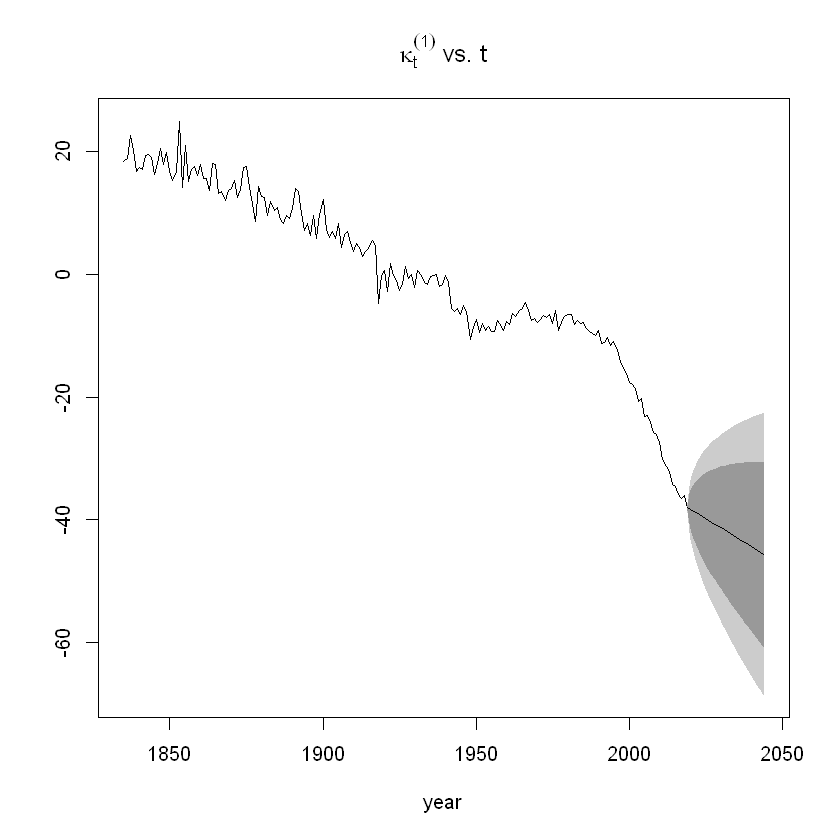
\includegraphics[scale =0.5]{output_24_1.png}
\end{figure}
\end{frame}

\begin{frame}{Projection des Taux de mortalité avec forecast}
\begin{figure}[!htb]
    \centering
    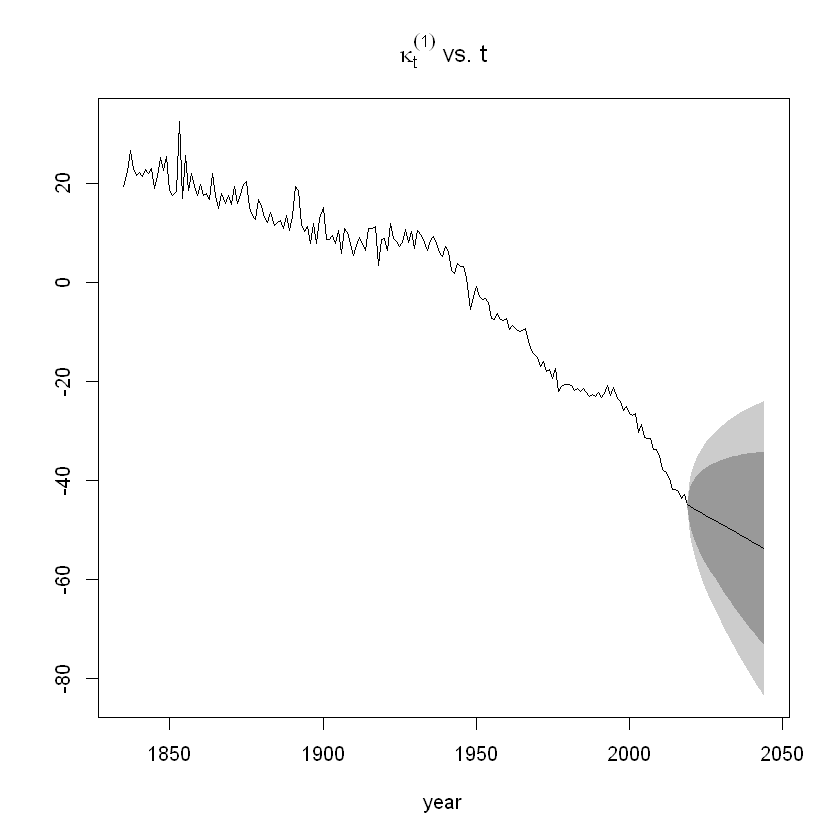
\includegraphics[scale =0.5]{output_24_2.png}
\end{figure}
\end{frame}

\begin{frame}{Projection des Taux de mortalité avec forecast}
\begin{figure}[!htb]
    \centering
    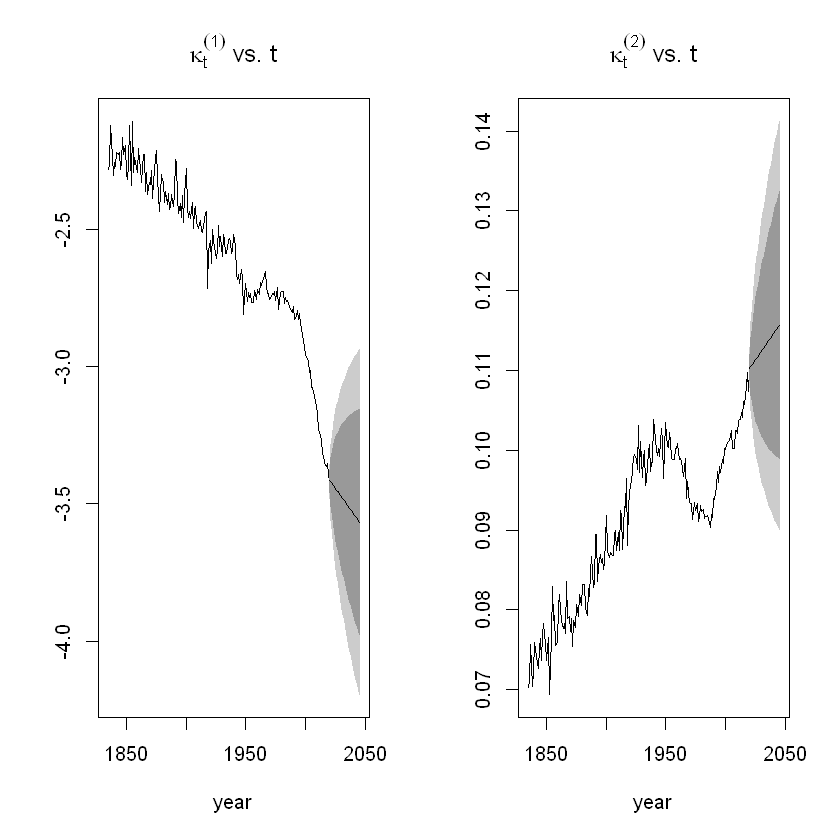
\includegraphics[scale =0.5]{output_25_0.png}
\end{figure}
\end{frame}

\begin{frame}{Projection des Taux de mortalité avec forecast}
\begin{figure}[!htb]
    \centering
    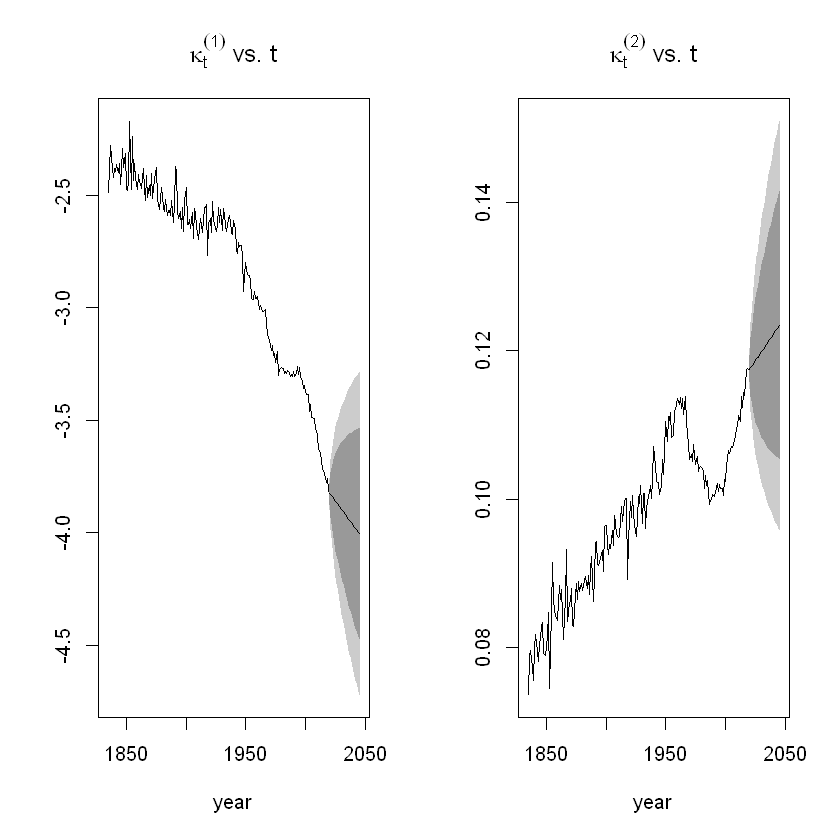
\includegraphics[scale =0.5]{output_25_1.png}
\end{figure}
\end{frame}

\begin{frame}{Conclusion}
CBD est plus performant pour les cohortes possédant un age plutôt avancé. 
\\Utilisation du modèle CBD pour la projection des taux de mortalité s'il s'agit d'une population agé et la durée de projection n'est pas assez large.
\\CBD a présenté un intervale de confiance moin large que celui de Lee-Carter, mais cet intervalle couvre une période plus vaste au niveau du CBD que celui du Lee-Carter.
\end{frame}

\end{document}